\chapter{Question 3}
\label{available-representation}

\textbf{Re-download the 1000 TimeMaps from A2, Q2.  Create a graph where the x-axis represents the 1000 TimeMaps.  If a TimeMap has ``shrunk'', it will have a negative value below the x-axis corresponding to the size difference between the two TimeMaps.  If it has stayed the same, it will have a ``0'' value.  If it has grown, the value will be  positive and correspond to the increase in size between the two TimeMaps.\\\\
As always, upload all the TimeMap data.  If the A2 github has the  original TimeMaps, then you can just point to where they are in  the report. }\\\\

Following are the steps I have taken to solve the problem:
\begin{itemize}
\item I repeated the same process that I did in Assignment 2 for getting the mementos data.
\item With the help of ODU Memento Aggregator, I downloaded TimeMaps for all the URIs that are extracted in Assignment 2 question 1 using the following curl command:\\
{\url {curl -i --silent http://mementoproxy.cs.odu.edu/aggr/timemap/link/1/<uri>}}\\
These URIs are located at \url{https://github.com/majetisiri/cs532-s16/blob/master/a2/uri.json}.
\item  I stored the output produced by the cURL command into a file `PagesList'. 
\item I processed the data from the above file to create a JSON with the original URI, memento URI , datetime and memento count. The memento count for each URI is derived by counting the URIs with rel=``memento''. This is outlined in Listing \ref{lst:q3code1}.
\item Using `getTimeMaps.py' I wrote the memento count for all the 1000 URIs for Assignment 2 and Assignment 10 in 2 different files `allMementosA2' and `allMementosA10' respectively.This code is listed in Listing \ref{lst:q3code2}.
\item I calculated the difference between TimeMaps for Assignment 10 and Assignment 2 and stored the output in `differenceTimemaps'. This code is illustrated in Listing \ref{lst:q3code3}
\item The output graph where the x-axis represents the 1000 TimeMaps is illustrated in Figure \ref{fig:q3fig1}. 
\begin{figure}[h!]
\begin{center}
\hspace*{-3cm} 
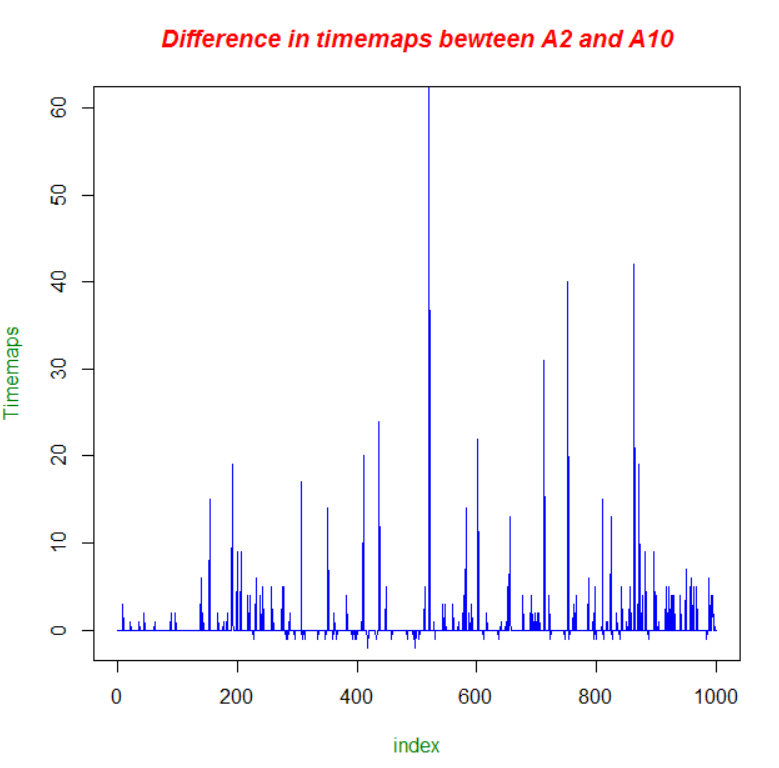
\includegraphics[scale=0.55, keepaspectratio=true]{figures/1.PNG}
\caption{Output graph with time maps on x axis}
\label{fig:q3fig1}
\end{center}
\end{figure}
\item From this graph we can conclude that most of the TimeMaps are `grown' as the value is positive. But we can see few TimeMaps are `shrunk' which have negative values.
\end{itemize}

\newpage
\textbf{Code Listing}
\sloppy
\lstinputlisting[language=Python,caption= Python code for getting mementos data.,frame=single,breaklines=true,label=lst:q3code1, tabsize=2, captionpos=b,numbers=left,showspaces=false,showstringspaces=false,basicstyle=\footnotesize]{src/getMementosData.py}


\textbf{Code Listing}
\sloppy
\lstinputlisting[language=Python,caption=python code for getting time maps from mementos data.,frame=single,breaklines=true,label=lst:q3code2, tabsize=2, captionpos=b,numbers=left,showspaces=false,showstringspaces=false,basicstyle=\footnotesize]{src/getTimeMaps.py}

\newpage
\textbf{Code Listing}
\sloppy
\lstinputlisting[language=Python,caption=python code for getting difference in time maps for mementos in Assignment 2 and Assignment 10.,frame=single,breaklines=true,label=lst:q3code3, tabsize=2, captionpos=b,numbers=left,showspaces=false,showstringspaces=false,basicstyle=\footnotesize]{src/getDifference.py}
